%%% LaTeX Template: Article/Thesis/etc. with colored headings and special fonts
%%%
%%% Source: http://www.howtotex.com/
%%% Feel free to distribute this template, but please keep to referal to http://www.howtotex.com/ here.
%%% February 2011
%%%
%%% Modified January 2016 by CDM

%%%  Preamble
\documentclass[11pt,letterpaper]{article}
\usepackage[margin=1.0in]{geometry}
\usepackage[T1]{fontenc}
\usepackage[bitstream-charter]{mathdesign}
\usepackage[latin1]{inputenc}					
\usepackage{amsmath}						
\usepackage{xcolor}
\usepackage{cite}
\usepackage{hyphenat}
\usepackage{graphicx}
\usepackage{float}
\usepackage{subfigure}
\usepackage{sectsty}
\usepackage[compact]{titlesec} 
\usepackage[tablegrid]{vhistory}
\usepackage{pbox}
\allsectionsfont{\color{accentcolor}\scshape\selectfont}

%%% Definitions
\definecolor{accentcolor}{rgb}{0.0,0.0,0.5} 
\newcommand{\teamname}{Team Name}
\newcommand{\productname}{Product Name}
\newcommand{\coursename}{CSE 4316: Senior Design I}
\newcommand{\semester}{Fall 2015}
\newcommand{\docname}{Architectural Design Specification}
\newcommand{\department}{Department of Computer Science \& Engineering}
\newcommand{\university}{The University of Texas at Arlington}
\newcommand{\authors}{Alan Turing \\ Grace Hopper \\ John Von Neumann \\ Ada Lovelace \\ Charles Babbage}

%%% Headers and footers
\usepackage{fancyhdr}
	\pagestyle{fancy}						% Enabling the custom headers/footers
\usepackage{lastpage}	
	% Header (empty)
	\lhead{}
	\chead{}
	\rhead{}
	% Footer
	\lfoot{\footnotesize \teamname \ - \semester}
	\cfoot{}
	\rfoot{\footnotesize page \thepage\ of \pageref{LastPage}}	% "Page 1 of 2"
	\renewcommand{\headrulewidth}{0.0pt}
	\renewcommand{\footrulewidth}{0.4pt}

%%% Change the abstract environment
\usepackage[runin]{abstract}			% runin option for a run-in title
%\setlength\absleftindent{30pt}			% left margin
%\setlength\absrightindent{30pt}		% right margin
\abslabeldelim{\quad}	
\setlength{\abstitleskip}{-10pt}
\renewcommand{\abstractname}{}
\renewcommand{\abstracttextfont}{\color{accentcolor} \small \slshape}	% slanted text

%%% Start of the document
\begin{document}

%%% Cover sheet
{\centering \huge \color{accentcolor} \sc \textbf{\department \\ \university} \par}
\vspace{1 in}
{\centering \huge \color{accentcolor} \sc \textbf{\docname \\ \coursename \\ \semester} \par}
\vspace{0.5 in}
\begin{figure}[h!]
	\centering
   	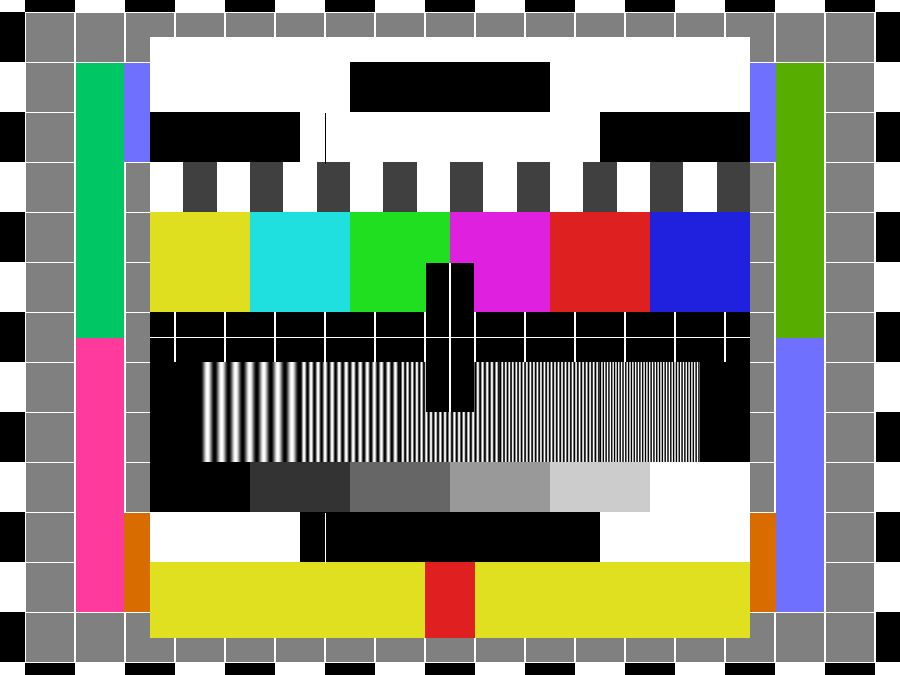
\includegraphics[width=0.60\textwidth]{images/test_image}
\end{figure}
\vspace{0.5 in}
{\centering \huge \color{accentcolor} \sc \textbf{\teamname \\ \productname} \par}
\vspace{0.5 in}
{\centering \large \sc \textbf{\authors} \par}
\newpage


%\vspace{1 in}
%\centerline{January 13th, 2012}
%\newpage

%%% Revision History
\begin{versionhistory}
  	\vhEntry{0.1}{10.01.2015}{GH}{document creation}
  	\vhEntry{0.2}{10.05.2015}{AT|GH}{complete draft}
  	\vhEntry{0.3}{10.12.2015}{AT|GH}{release candidate 1}
  	\vhEntry{1.0}{10.20.2015}{AT|GH|CB}{official release}
  	\vhEntry{1.1}{10.31.2015}{AL}{added design review requests}
\end{versionhistory}
\newpage

%%% Table of contents
\setcounter{tocdepth}{2}
\tableofcontents
\newpage

%%% List of figures and tables (optional)
\listoffigures
\listoftables
\newpage

%%% Document sections
\section{Introduction}
The Smart Hospital Management Tools website is meant to combine multiple pages in order to allow the Smart Hospital to manage their information in one place. The website is meant to fuflfill key requirements, such as allowing simulations to be scheduling, managing inventory logs, create events and displaoy them on a calendar, and allow the user to log in and log out.
\newpage
\section{System Overview}
Lorem ipsum dolor sit amet, quidam omnesque ea vis. Eum an aliquip legendos recusabo. Mea ex purto natum, ne movet fuisset sit. Labore audiam eos ad, facer ornatus posidonium ne ius, et eos duis delenit nusquam.
\newpage
\section{Subsystem Definitions \& Data Flow}
This section breaks down the layer abstraction to another level of detail. 

\begin{figure}[h!]
	\centering
 	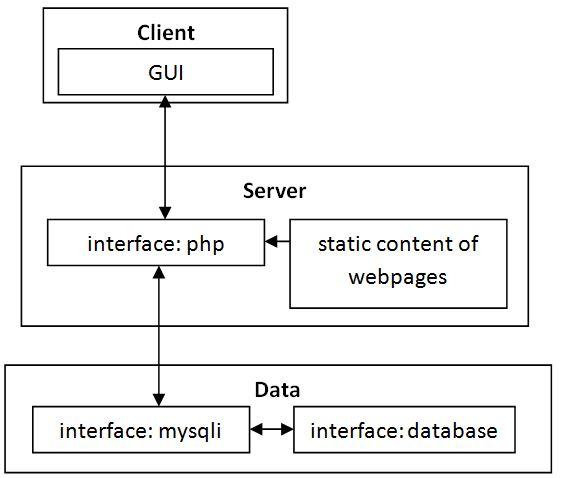
\includegraphics[width=\textwidth]{images/LayerBlockDiagramWithSubsystems}
 \caption{A simple data flow diagram}
\end{figure}

\newpage
\section{X Layer Subsystems}
In this section, the client layer is described in terms of the software design.


\subsection{Layer Software Dependencies}
The client layer requires a browser to be operated by the user.

\subsection{Calendar}
The calendar subsystem displays events.

\begin{figure}[h!]
	\centering
 	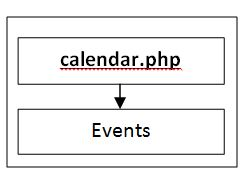
\includegraphics[width=0.40\textwidth]{images/calendar}
 \caption{Calendar Subsystem Diagram}
\end{figure}

\subsubsection{Subsystem Software Dependencies}
The calendar subsystem requires a browser to operated by the user.

\subsubsection{Subsystem Programming Languages}
The calendar subsystem requires html, css, and javascript.


\subsection{Dashboard}
The dashboard subsystem allows users to create events.

\begin{figure}[h!]
	\centering
 	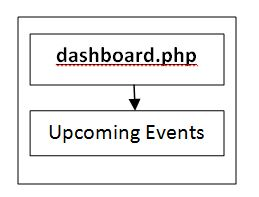
\includegraphics[width=0.40\textwidth]{images/dashboard}
 \caption{Dashboard Subsystem Diagram}
\end{figure}


\subsubsection{Subsystem Software Dependencies}
The dashboard subsystem requires a browser to operated by the user.

\subsubsection{Subsystem Programming Languages}
The dashboard subsystem requires html, css, and javascript.


\subsection{Management}
The management subsystem allows for administrative duties including changing user permission level, accepting new accounts, approving events, and generating reports.

\begin{figure}[h!]
	\centering
 	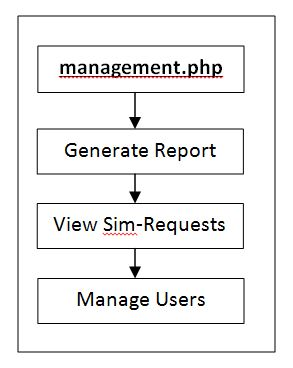
\includegraphics[width=0.40\textwidth]{images/management}
 \caption{Management Subsystem Diagram}
\end{figure}


\subsubsection{Subsystem Software Dependencies}
The management subsystem requires a browser to operated by the user.

\subsubsection{Subsystem Programming Languages}
The management subsystem requires html, css, and javascript.




\subsection{Inventory}
The inventory subsystem allows for searching, inserting, deletion, and editing of the inventory table.

\begin{figure}[h!]
	\centering
 	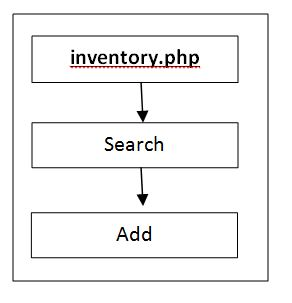
\includegraphics[width=0.40\textwidth]{images/inventory}
 \caption{Inventory Subsystem Diagram}
\end{figure}



\subsubsection{Subsystem Software Dependencies}
The inventory subsystem requires a browser to operated by the user.

\subsubsection{Subsystem Programming Languages}
The inventory subsystem requires html, css, and javascript.





\newpage
\section{Y Layer Subsystems}
In this section, the layer is described in some detail in terms of its specific subsystems. Describe each of the layers and its subsystems in a separate chapter/major subsection of this document. The content of each subsystem description should be similar. Include in this section any special considerations and/or trade-offs considered for the approach you have chosen.

\subsection{Subsystem 1}
This section should be a general description of a particular subsystem for the given layer. For most subsystems, an extract of the architectural block diagram with data flows is useful. This should consist of the subsystem being described and those subsystems with which it communicates.

\begin{figure}[h!]
	\centering
 	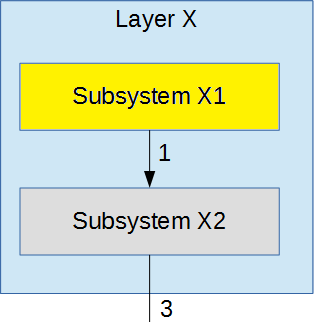
\includegraphics[width=0.60\textwidth]{images/subsystem}
 \caption{Example subsystem description diagram}
\end{figure}

\subsubsection{Assumptions}
Any assumptions made in the definition of the subsystem should be listed and described. Pay particular attention to assumptions concerning interfaces and interactions with other layers.

\subsubsection{Responsibilities}
Each of the responsibilities/features/functions/services of the subsystem as identified in the architectural summary must be expanded to more detailed responsibilities. These responsibilities form the basis for the identification of the finer-grained responsibilities of the layer's internal subsystems. Clearly describe what each subsystem does.

\subsubsection{Subsystem Interfaces}
Each of the inputs and outputs for the subsystem are defined here. Create a table with an entry for each labelled interface that connects to this subsystem. For each entry, describe any incoming and outgoing data elements will pass through this interface.

\begin {table}[H]
\caption {Subsystem interfaces} 
\begin{center}
    \begin{tabular}{ | p{1cm} | p{6cm} | p{3cm} | p{3cm} |}
    \hline
    ID & Description & Inputs & Outputs \\ \hline
    \#xx & Description of the interface/bus & \pbox{3cm}{input 1 \\ input 2} & \pbox{3cm}{output 1}  \\ \hline
    \#xx & Description of the interface/bus & \pbox{3cm}{N/A} & \pbox{3cm}{output 1}  \\ \hline
    \end{tabular}
\end{center}
\end{table}

\subsection{Subsystem 2}
Repeat for each subsystem

\subsection{Subsystem 3}
Repeat for each subsystem


\newpage
\section{Z Layer Subsystems}
In this section, the Database Layer is described in some detail n terms of its specific subsystems.

\subsection{Database Tables}
The Database Tables Subsystem is what provides the database with all the needed information for the website. This data is connected through HTML and PHP code to gather information from the tables or even put data back into the tables properly. This allows for proper storage of information to the database so that the website portion may run smoothly and without any error or incorrect information when sought by a user.

\begin{figure}[h!]
	\centering
 	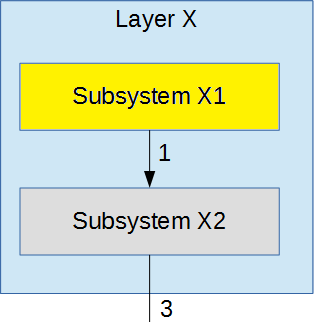
\includegraphics[width=0.60\textwidth]{images/subsystem}
 \caption{Example subsystem description diagram}
\end{figure}

\subsubsection{Assumptions}
The main assumption concerning the Database Tables was that it was an important part of the project to run efficiently.

\subsubsection{Responsibilities}
The Database Tables were a significant portion of the project. It stores everything needed for the actual website to display some sort fo information without hard coding data into fields. The Database Tables needed to be correct and also be connected to one each other to extract information from multiple tables and make sure that the information needed was the correct information that is being sent. This ensured any communication with the website server and database went successfully and provided the correct info needed.

\subsubsection{Subsystem Interfaces}
Each of the inputs and outputs for the subsystem are defined here. Create a table with an entry for each labelled interface that connects to this subsystem. For each entry, describe any incoming and outgoing data elements will pass through this interface.

\begin {table}[H]
\caption {Subsystem interfaces} 
\begin{center}
    \begin{tabular}{ | p{1cm} | p{6cm} | p{3cm} | p{3cm} |}
    \hline
    ID & Description & Inputs & Outputs \\ \hline
    \#1 & CREATE DATABASE & \pbox{3cm}{Name of Database} & \pbox{3cm}{Database is created with given input name}  \\ \hline
    \#2 & CREATE TABLE & \pbox{3cm}{Name of Table} & \pbox{3cm}{Table is created in current Database}  \\ \hline
    \#3 & INSERT TO and VALUES & \pbox{3cm}{Table's Column's Names and Values} & \pbox{3cm}{Information filled tables}  \\ \hline
    \end{tabular}
\end{center}
\end{table}

\newpage

%%% References
\bibliographystyle{plain}
\bibliographystyle{reference/IEEEtran_custom}
\bibliography{reference/refs}{}

\end{document}